\documentclass{standalone}

% Adapted from Kognity
\begin{document}

\section{Sources of Finance}

\subsection{The Role of Finance}
There are many things companies spend money on. 
This subsection will list some of the uses of finance.

\paragraph{Capital Expenditure}
One of the most common source of expenditure is \texttt{Capital}.
Capital investment is spending money on \texttt{fixed assets}, which are assets that are hard to sell.
Generally, capital expenditures are used to fund long term goals, such as building facilities or buying machinery.
Capital expenditures are often funded by long term sources of finance.

\paragraph{Revenue Expenditure}
Revenue expenditure is spending money on general operation costs.
Expenditures such as wages or rent.
Revenue expenditures are often funded by short to medium term sources of finance.
When a firm cannot pay its revenue expenditure, they go into a state of insolvency.

\subsection{Internal Source of Finance}
Internal sources of finance refers to money collected internally.
Such as the sale of assets, retain profit, or personal funds.

\begin{description}
    \item[Personal Funds] is the money invested by the owners of the business
    \item[Retained Profit] is profit leftover (after paying the bills) from end of a trading year
    \item[Sale of Assets] is money gained from selling any assets
\end{description}

\subsection{External Source of Finance}
Opposite to Internal Sources of Finance, External Sources of Finance is money gathered through outside means.

\subsubsection{Equity Finance}
Equity Finance is money gathered by selling ownership of the company.
Equity does not come with any interest, or requirement of repayment.
However, selling equity comes with the cost of losing control and dividends.

\begin{description}
    \item[Share Capital] is money raised through selling shares
    \item[Business Angel] are wealthy investors, often buying a chunk of shares as investment
    \item[Venture Capitalist] are companies similar to Business Angels
\end{description}

\subsubsection{Debt Finance}
Debt finance is the method of borrowing money to acquire finance.
Often times, borrowing money can quickly bring money for investment, but their is the cost of interest.
Interest is additional money owed overtime as borrowed money is payed off.

\begin{description}
    \item[Loan Capital] are long term borrowing of money, often for the purchasing capital. These loans require collateral in case there is a default on the loan.
    \item[Overdrafts] are a high cost, short term loan. It is when the company spend more money that they have in their account, and have to pay back in high interest.
    \item[Credit Cards] are a method of borrowing money and paying back every month.
\end{description}

\subsubsection{Financial Aid}
Financial Aid is money given to the companies for free.
Generally, these come from NGOs or governments who want to support the business.

\begin{description}
    \item[Subsidies] money given to the production of goods that is good for the society, often provided by the government
    \item[Grants] are loans with no interest, and does not need to be paid back. There may be conditions on how the money is spent
\end{description}

\subsubsection{Other Sources of Finance}
Other then the main sources of finance, there are others that does not fit the groups.

\begin{description}
    \item[Trade Credit] is a method of paying for goods at a later date, without interest. Often provided to companies by companies.
    \item[Debt Factoring] is the action of selling debt, to a debt factoring company. Often at a lower cost, but with an immediate payment.
    \item[Leasing] is the action of leasing fixed assets instead of buying them. Flexible, but cost more in the long run.
\end{description}

\subsection{Short, Medium, and Long-Term Finance}
External sources of finance can be broken into 3 types according to their durations.
Internal sources of finance can be fall into any of these categories.

\subsubsection{Short-Term}
Short-term finance are repaid within 12 months. 
These are normally used to solve cash flow problems or to pay for revenue expenditure.
Short-term finance is often expensive and have high interest.

Below is a list of short term finances:
\begin{itemize}
    \item Overdraft
    \item Trade Credit
    \item Debt Factoring
    \item Leasing
    \item Subsidies
\end{itemize}

\subsubsection{Medium-Term}
Medium-term finance last longer than 12 months, but less than 5 year.
These are normally used for buying fixed assets or capital.
Medium term finance is in-between of short and long term finance.

Below is a list of medium term finances:
\begin{itemize}
    \item Loan Capital
    \item Leasing
    \item Subsidies
\end{itemize}

\subsubsection{Long-Term}
Long term finance last longer than 5 years.
Mortgages and all equity finance belong in this category.

Below is a list of long term finance:
\begin{itemize}
    \item Share Capital
    \item Venture Capital
    \item Business Angel
    \item Loan Capital
    \item Grants
\end{itemize}

\subsection{Evaluation of Sources of Finance}
Often times, companies have to make decision on which source of finance to choose.
Different methods of finance have different purposes, with different opportunity cost and effectiveness.

There is three general idea for choosing sources of finance, \texttt{gearing}, \texttt{purpose}, and \texttt{ownership}.

\subsubsection{Gearing}
\textit{This will be further explained in 3.6, Efficiency Ratio Analysis.}

Gearing ratio calculates the percentage of loan capital versus the total capital of the business.
Having a high gearing ratio makes the company risky in case they default on their loans.
However, having a high gearing ratio lowers the amount of ownership that needs to be split.

\subsubsection{Purpose}
Consider the purpose of the funds when gathering finance.
Determine if the source of finance falls into short, medium, or long term groups.

\subsubsection{Ownership}
Different companies have access to different kinds of finance.
Sole traders and Partnerships have access to mostly internal sources of finance.
They can also take loans and use trade credit.
Bigger corporation generally cannot use personal funds, but can take advantage of equity for financing.

\section{Cost and Revenue}
In order for a business to make money, its revenue must be larger than its cost.
In this section, we will discuss the different cost and revenue of a company.

\subsection{Classification of Costs}
Cost can be split up into two major categories, Fixed Cost and Variable Costs.

\subsubsection{Variable Cost}
Variable cost is cost that change directly due to production.
These include material and labor used for production.

\subsubsection{Fixed Costs}
Fixed cost is cost that is not effected directly with production.
For example, electricity bills remain relatively constant no matter the amount produced.
Although electrify is required to make the product, it is not effected directly by the amount produced.

Other fixed costs include rent, salaries, capital.

\subsection{Direct and Indirect Costs}
Costs can also be clarified into direct and indirect costs.
Direct costs are those that directly impact the good and service a company produces.
For example, raw material is a direct cost, but coffee machine refills are an indirect cost.

Examples of direct costs are salary or utility, while examples indirect costs are infrastructure cost and advertising.

\section{Revenue and Revenue Streams}
Revenue is the money earned from the selling of goods and services.
It is different than profit, in that profit is revenue minus cost.
Simply, revenue can be calculated by the selling price of a product times the amount sold.

Revenue streams are methods of generating revenue.
Many companies do not earn money from one source.
For example, a movie theater do not earn money just from selling tickets, but also food and drinks.
Or newspapers that do not earn money just from selling newspapers, but also from advertisements.

\section{Break-Even Analysis}
In order to maintain a health revenue and cost relationships, many companies use break even analysis plan ahead.
Break even analysis allows a company to find how much it need to sell in order to \texttt{break even} (profit is greater than zero).

\subsection{Calculating the Break-Even Point}
There are several units used in the calculation that have to be noted.

\begin{description}
    \item[Fixed Cost] is cost not effected by change of production
    \item[Variable Cost] is cost directly effected by change of production
    \item[Contribution per Unit] is the price per unit minus the variable cost per unit
    \item[Break Even Point] is the unit of product sold that the total profit is zero
    \item[Margin of Safety] is the difference between the current unit sold and the break even point
\end{description}

The break even point can be calculated using the following equation:
\begin{equation}
    \frac{\textrm{Fixed Costs}}{\textrm{Contribution per Unit}} 
\end{equation}

\subsection{Break-Even Charts}
Break even chart shows the break even point against unit sold and profit.
The x axis is output, or the amount sold.
The y axis is revenue and cost.

There are three lines.
The first line is the Fixed Cost, which is a parallel line with equation $y=t\texttt{fixed cost}$.
The second line is the Total Cost, which starts at the fixed cost, and increase over time.
It's equation is $y = \texttt{variable cost per unit} \cdot x + \texttt{fixed cost}$.
The last line is the Total Revenue, which starts at zero.
It has the equation $y = \texttt{contributions per unit} \cdot x$

The point at which Total Revenue intersects Total cost is the break even point.
Draw a line from the Break even point to the x axis.
The difference between the break even point and the actual output is the margin of safety.

\subsection{Evaluation of Break-Even Analysis}
Break even analysis is easy to use, and show the important information that keeps the company alive.
A company can use break even analysis predict how changes in production can change the profit levels.
However, break even analysis is not very accurate. 
It ignores a companies' inventory and economies of scale. 
It assumes all products are sold at the same price.

\section{Final Accounts}
In order for business to understand what is going on in their company, they often gather data to create a final account.
A final account provides insight into the finance of the company overall.
Final accounts are created periodically, often at the end of a business year.
However, note that final account only accounts for the business at their current state. 
What happens in the future is not factored in.

\subsection{Purpose of Final Account to Stakeholders}
Internal stakeholders often look to final accounts for information about the company's health.
Management might look at the final account for planning and organizing.
While employees might look at a final account to see the financial stability of a company.

External stakeholders look at the final accounts for different reasons.
The government may look into the final accounts to make sure the company is following regulations and paying taxes.
Competitors may look into the final accounts to compare profits and financial strength.

\subsection{Ethics in Accounting}

\subsection{Profit and Loss Account}
\begin{itemize}
    \item Sales Revenue
    \item Cost of Good Sold
    \item Gross Profit
    \item Expenses
    \item Total Expense
    \item Net Profit before Interest and Tax
    \item Interest
    \item Net Profit before Tax
    \item Tax
    \item Net Profit After Interest and Tax
    \item Dividends
    \item Retained Profit
\end{itemize}

\subsection{Balance Sheet}
\begin{itemize}
    \item Fixed Assets
        \begin{itemize}
            \item Fixed Assets
            \item Accumulated Depreciation
            \item Net Fixed Assets
        \end{itemize}
    \item Current Assets
        \begin{itemize}
            \item Cash
            \item Debtors
            \item Stock
            \item Total Current Assets
        \end{itemize}
    \item Current Liabilities
        \begin{itemize}
            \item Overdraft
            \item Creditors
            \item Short Term Loans
            \item Total Current Liabilities
            \item Net Current Assets
            \item Total Assets less Current Liabilities
        \end{itemize}
    \item Long Term Liabilities (Debt)
        \begin{itemize}
            \item Long-Term Loans
            \item Mortgage
            \item Total Long-Term Liabilities
            \item Net Assets
            \item Equity
        \end{itemize}
\end{itemize}

\subsection{Figures}
\begin{figure}[h]
\begin{center}
	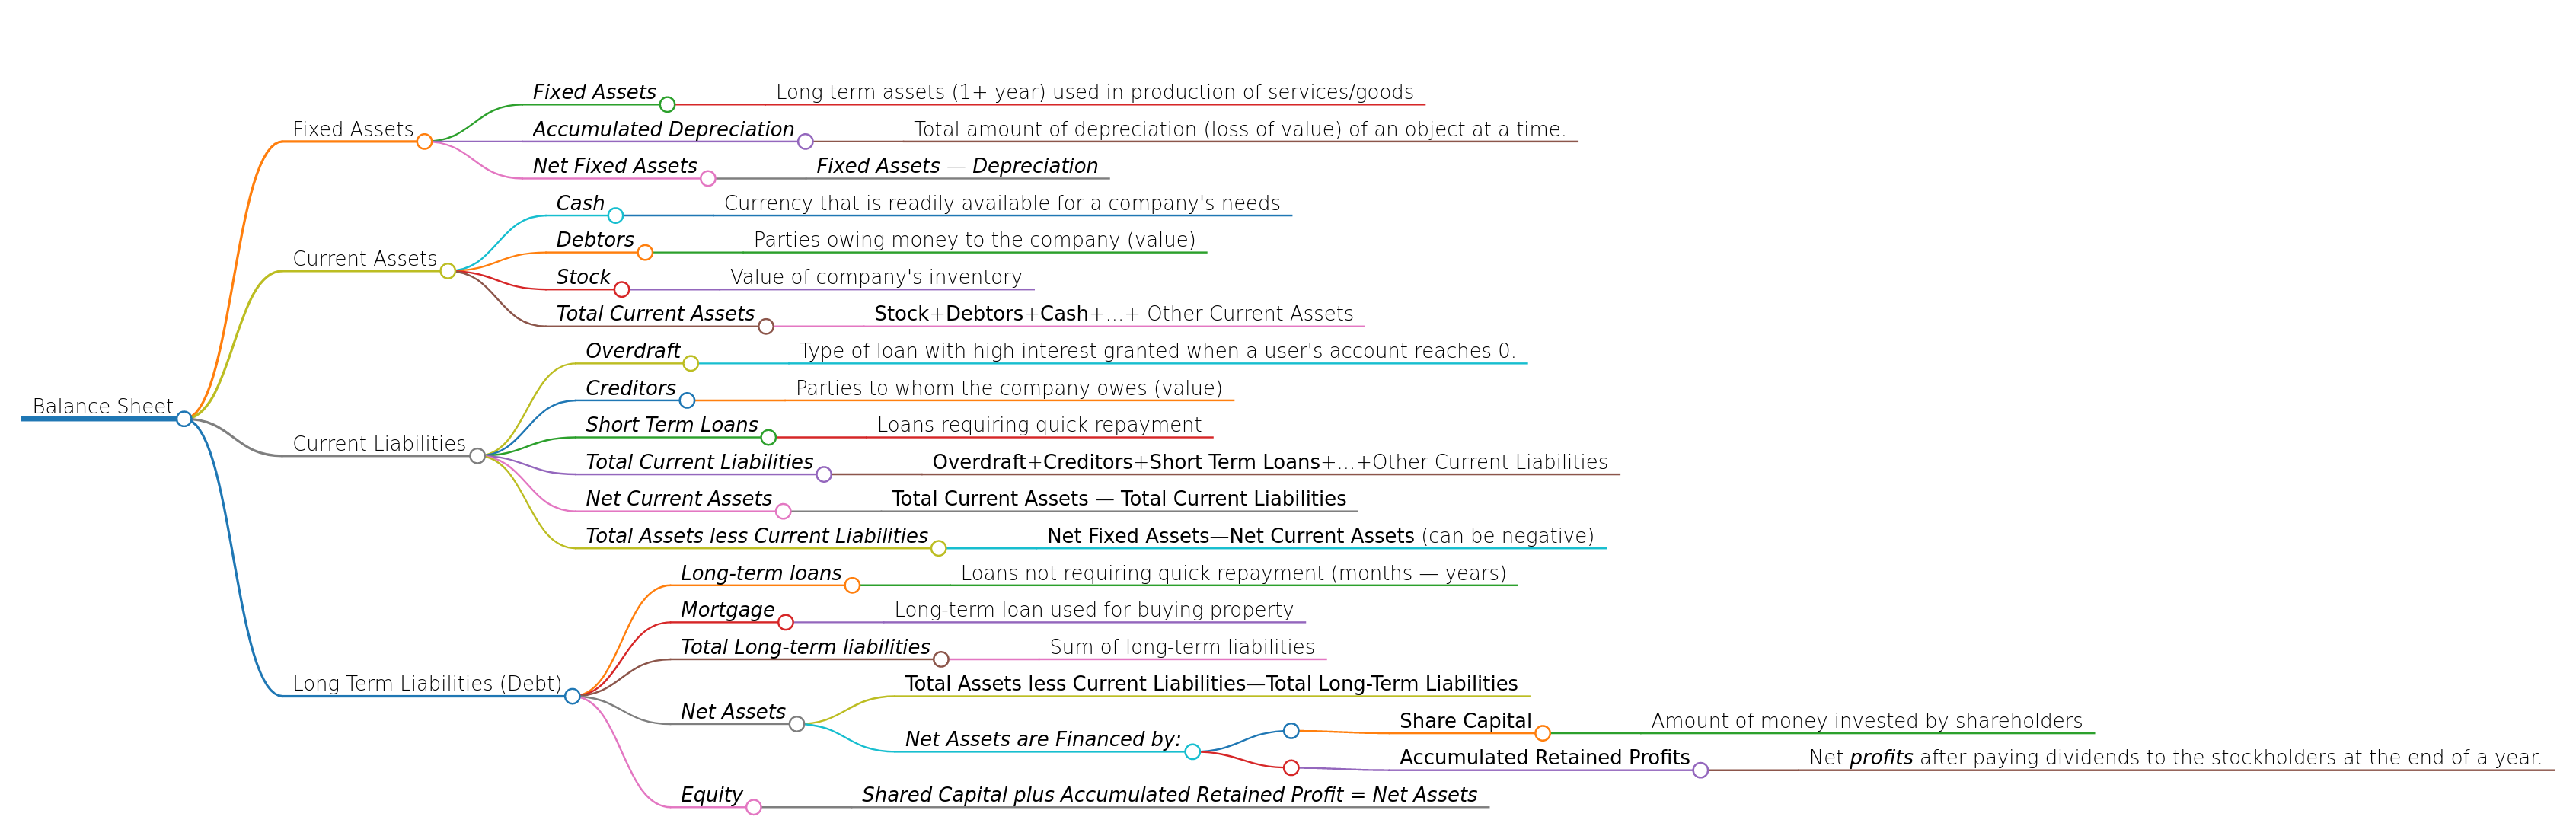
\includegraphics[width=\textwidth]{./figures/unit 3/bs.png}
	\caption{Balance Sheet}
\end{center}
\end{figure}

\begin{figure}[h]
\begin{center}
	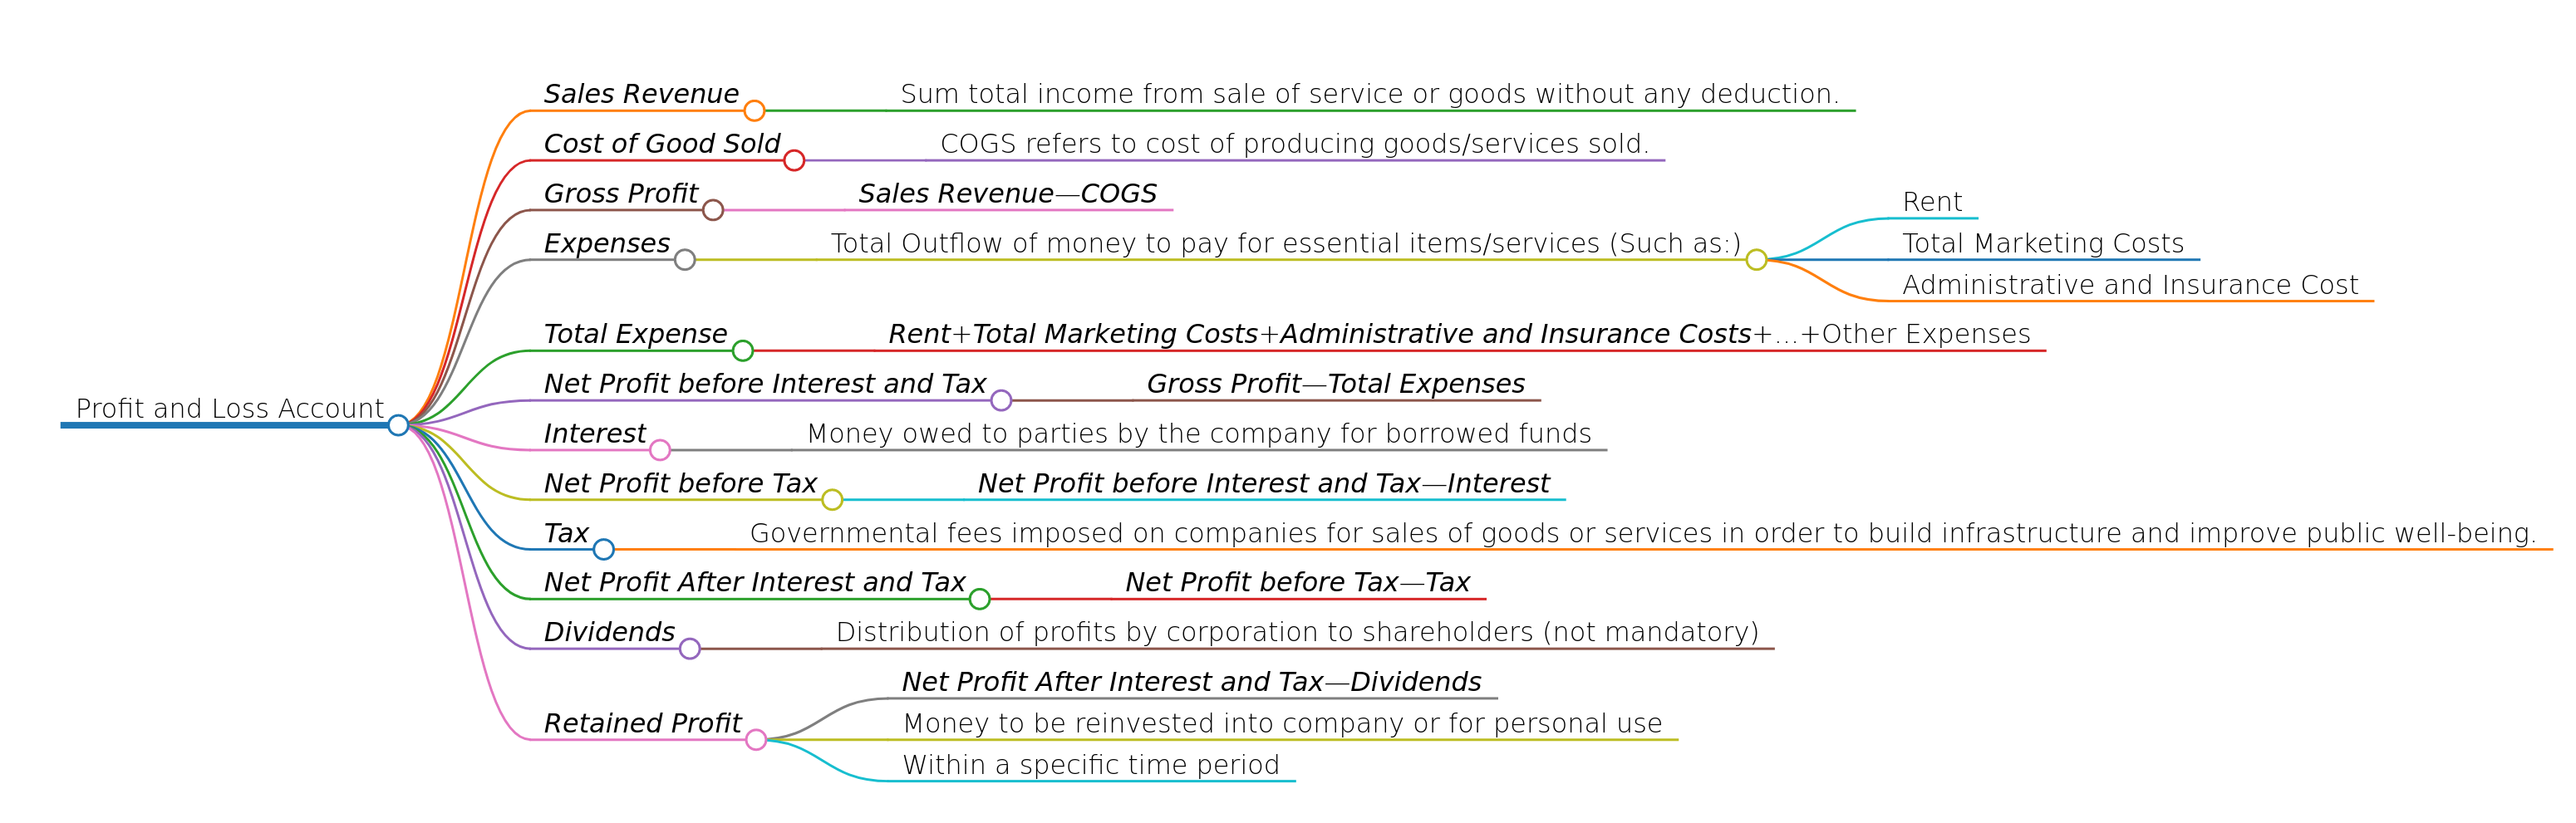
\includegraphics[width=\textwidth]{./figures/unit 3/pl.png}
	\caption{Profit and Loss Account}
\end{center}
\end{figure}

\subsection{Intangible Assets}
Although we can calculate a value for most assets, some assets have intangible value.
\begin{description}
    \item[Patents] are legal protection that protects an invention for a set number of years.
    \item[Copyright] are similar to patents, but for artistic works
    \item[Brand] is the brand image of a company
    \item[Registered Trademark] is a distinctive symbol of the company.
    \item[Goodwill] is the difference between the purchasing price of a company and its net assets
\end{description}

\subsection{Depreciation}
Over time, fixed assets decrease in value.
It is often hard to sell something at the same value as you bought it, especially after a few years.

\subsubsection{Causes of Depreciation}
Often times, depreciation is caused by wear and tear.
Capital such as factories or equipment will get older over time, be prone to breaking.
This decrease the value of the fixed asset.

Another cause is obsolescence.
This happens when newer technology arrives, and render the current product outdated.
In this case, the fixed asset will also decrease in value.

\subsubsection{Calculating Depreciation}
IB supports two methods of calculations depreciation:
The Straight Line method and Reducing Balance method.

The straight line method assumes the asset decrease in value at a fixed rate.
Use this equation to calculate the decrease in value per unit of time.
\begin{equation}
    \textrm{Depreciation per unit of time} = \frac{\textrm{Purchase Price} - \textrm{Residual Value}}{\textrm{Estimated useful life}}
\end{equation}

The Reducing Balance method assumes the asset reduce in value by a percent of its value.

The straight line method is easier to calculate, and easy to plan around.
However, it is not as accurate as the reducing balance method.

\section{Profitability and Liquidity Ratio Analysis}

\subsection{Profitability and Efficiency Ratio}
Profitably ratios measures how efficient a company can use its resources to make money.

\subsubsection{Gross Profit Margin (GPM)}
GPM is a measure of how profitable the core business activities are.
It is calculate with the following equation:
\begin{equation}
    GPM = \frac{\textrm{Gross Profit}}{\textrm{Sales Revenue}} \times 100\%
\end{equation}

The higher the ratio, the more the business earn from is revenue.
There is no good ratio, as different companies have different ideal ratios.
Restaurants, for example, generally have lower GPM ratios while tech based companies have higher GPM ratios.

In order to improve GPM, one can change the price of the product.
The higher the price the more the company can earn per product.
However, be aware that changing the price can also effect the amount sold.
A company can also look to reducing cost.

\subsubsection{Net Profit Margin (NPM)}
Net Profit Margin shows net profit as a percentage of sales revenue.
Similar to GPM, but factor into fixed costs.
Calculate NPM with the following equation:
\begin{equation}
    NPM = \frac{\textrm{Net profit before interest and tax}}{\textrm{Sales revenue}} \times 100\%
\end{equation}

The higher the ratio, the better the company is at managing overhead costs.

You can increase NPM Similar to GPM, but additionally decrease operation costs.

\subsubsection{Return On Capital Employed (ROCE)}
Return On Capital Employed measures how well a company can make money from capital.
Use the following equation to calculate ROCE.
\begin{equation}
    ROCE = \frac{\textrm{Net profit before interest and tax}}{\textrm{Capital Employed}} \times 100\%
\end{equation}
In which \texttt{Capital Employed} can be calculated with the equation below:
\begin{equation}
    \textrm{Capital Employed} = \texttt{Long Term Liabilities} + \texttt{Share Capital} + \texttt{Retained Profits}
\end{equation}

The higher ROCE is, the better the company is at making money from capital.
Note that if ROCE is lower than the interest rate of a risk-free saving account, then a company is often not worth investing into.

In order to increase ROCE, a company can increase NPM.
They can also reduce long term liabilities.

\subsection{Liquidity Ratios}
Liquidity ratio measures how well can a company sell its assets.
They can measure how well can a company pay off short term debts.

\subsubsection{Current Ratio}
Current ratio measures how much a company own compared to how much they owe.
Calculate the current ratio with the equation below:
\begin{equation}
    \texttt{Current Ratio} = \frac{\textrm{Current Assets}}{\textrm{Current Liabilities}}
\end{equation}

The higher the ratio, the healthier the company's total assets.
Note, companies want their current ratio to be above 1, as dropping below 1 means they do not have enough assets to pay off their debts.
However, if the current ratio is too high, then the company is at risk of wasting the money accumulated.
Different types of business have different current ratios.
For example, if a company have a steady cash flow, it is not as worried about gathering money to pay debts, and can live with a lower current ratio.

To improve the current ratio, a company can reduce its current liabilities.
They can also increase their credit system and sell unused fixed assets.
Decreasing overheads and negotiating for longer payment terms can also improve the current ratio.

\subsubsection{Acid Test Ratio}
Acid Test Ratio measures a more severe indicator of a firm's ability to pay off short term debt, similar to the Current Ratio.
Stocks is subtracted from current asset, as it is not as liquid.
Use the equation below to calculate the Acid Test Ratio:
\begin{equation}
    \texttt{Acid Test Ratio} = \frac{\textrm{Current Assets} - \textrm{Stock}}{\textrm{Current Liabilities}}
\end{equation}

Evaluate this ratio similar to the current ratio.

To improve the acid test ratio, a company can improve the current ratio.
They can also increase sales, which can turn stock into current assets.

\section{Efficiency Ratio Analysis}
In this section, we will continue to look at ratios.
This section focuses on ratios that improve a company's efficiency.

\subsubsection{Stock Turnover Ratio}
The Stock Turnover Ratio measures frequent a company have to replenish its stocks.
The more frequent, the company is better at converting stocks into sales.
Use the equation below the calculate the Stock Turnover Ratio.
\begin{equation}
    \texttt{Stock Turnover Ratio} = \frac{\textrm{Cost of Goods Sold}}{\textrm{Average Stock}}
\end{equation}

The higher the Stock Turnover Ratio, the better the company is at turning stock into sales.
Note, Stock Turnover Ratio does not apply to every company, especially companies that sell services.

Companies can improve this ratio by:
\begin{itemize}
    \item Lowering price
    \item Increasing promotions
    \item Stocking fast selling items
    \item Buy stocks \textit{just in time}
    \item Use better sales forecast
\end{itemize}

\subsubsection{Debtor Days}
Debtor days measures how well a company can collect its debt.
Use the equation below to calculate Debtor Days:
\begin{equation}
    \texttt{Debtor Days} = \frac{\textrm{Debtors}}{\textrm{Total Sale Revenue}} \times 365
\end{equation}

Companies can increase Debtor Days by improving credit control.

\subsubsection{Creditor Days}
Creditor Days measures the number of days a company settle its debts.
Similar to Debtor Days, but for the company's debts.
Use the equation below to calculate Creditor Days:
\begin{equation}
    \texttt{Debtor Days} = \frac{\textrm{Creditors}}{\textrm{Cost of Goods Sold}} \times 365
\end{equation}

Companies can improve creditor days but having a good stock control system, and having good relations with suppliers.

\subsubsection{Gearing Ratio}
Gearing Ratio measures how much of a company's capital is funded by long term debt.
A normal gearing ratio would be between $25\%$ to $50\%$.
The higher the gearing ratio, the less control a company would have over itself.
Also, interest and dividend will be higher with a higher gearing ratio.

Calculate the gearing ratio with the equation below:
\begin{equation}
    \texttt{Gearing Ratio} = \frac{\textrm{Loan Capital}}{\textrm{Capital Employed}} \times 100\%
\end{equation}

To improve the gearing ratio, a company can increase retained profit.
They can also pay up long term loans or swap debt for equity.

\section{Cash flow}

\section{Investment Appraisal}

\section{Budgets}

\end{document}
